\documentclass[titlepage, 12pt]{scrartcl}
\usepackage[utf8]{inputenc}
\usepackage{setspace}
\usepackage{subcaption}
\doublespacing
\usepackage[margin=1in]{geometry}
\usepackage{graphicx}
\usepackage[nottoc,numbib]{tocbibind}

%%% Maketitle metadata
\newcommand{\horrule}[1]{\rule{\linewidth}{#1}} 	% Horizontal rule
        
\title{
		\vspace{-1in} 	
		\usefont{OT1}{bch}{b}{n}
		\normalfont \normalsize \textsc{University of California, Los Angeles \\
		180DB Winter 2019 Final Report \\
		Professor Pottie} \\ [25pt]
		\horrule{0.5pt} \\
		\Huge ZombieArcher \\
		\vspace{-.3in}
		\horrule{2pt} \\
		\vspace{1in}
}

\author{
        Sidharth Bambah (904 787 435)\\
        Sparsh Gauba (204 600 605)\\
        Andrew Juarez (504 572 352)\\
        Mohamed Shatela (604 644 424)\\\\
        \vspace{1in}
        }

\date{ \large March 2019}

\begin{document}

\maketitle
\tableofcontents
\newpage
\section{Project Overview}
    \subsection{Overall Game Design}
        The ZombieArcher project is an interactive augmented reality game which involves using a bow and arrow to fight zombie enemy AI. The purpose of the game is to create an interactive and immersive experience for the user in which the user's mastery of the game mechanics are transferable to real life archery skills. The game does so by providing the user with scenarios in which the user has to aim and shoot an arrow to reach a target at various locations, and both static and moving targets. To make in-game skills transferable to the real world, the physical controller emulates the basic functions of a bow and arrow, namely the vertical and lateral angle of launch and the initial kinetic energy of the arrow. Additionally, the arrow in the game environment is subject to gravitational force, so depending on the distance of the target, the user has a range of correct combinations of launch angle and initial kinetic energy of the arrow to choose from. By constantly assesses the user’s performance in terms of accuracy, precision and reaction time and collecting data regarding the user’s performance, the game adjusts the difficulty in each of the performance categories to help the user improve upon his or her weak points. 
        \begin{figure}
            \centering
            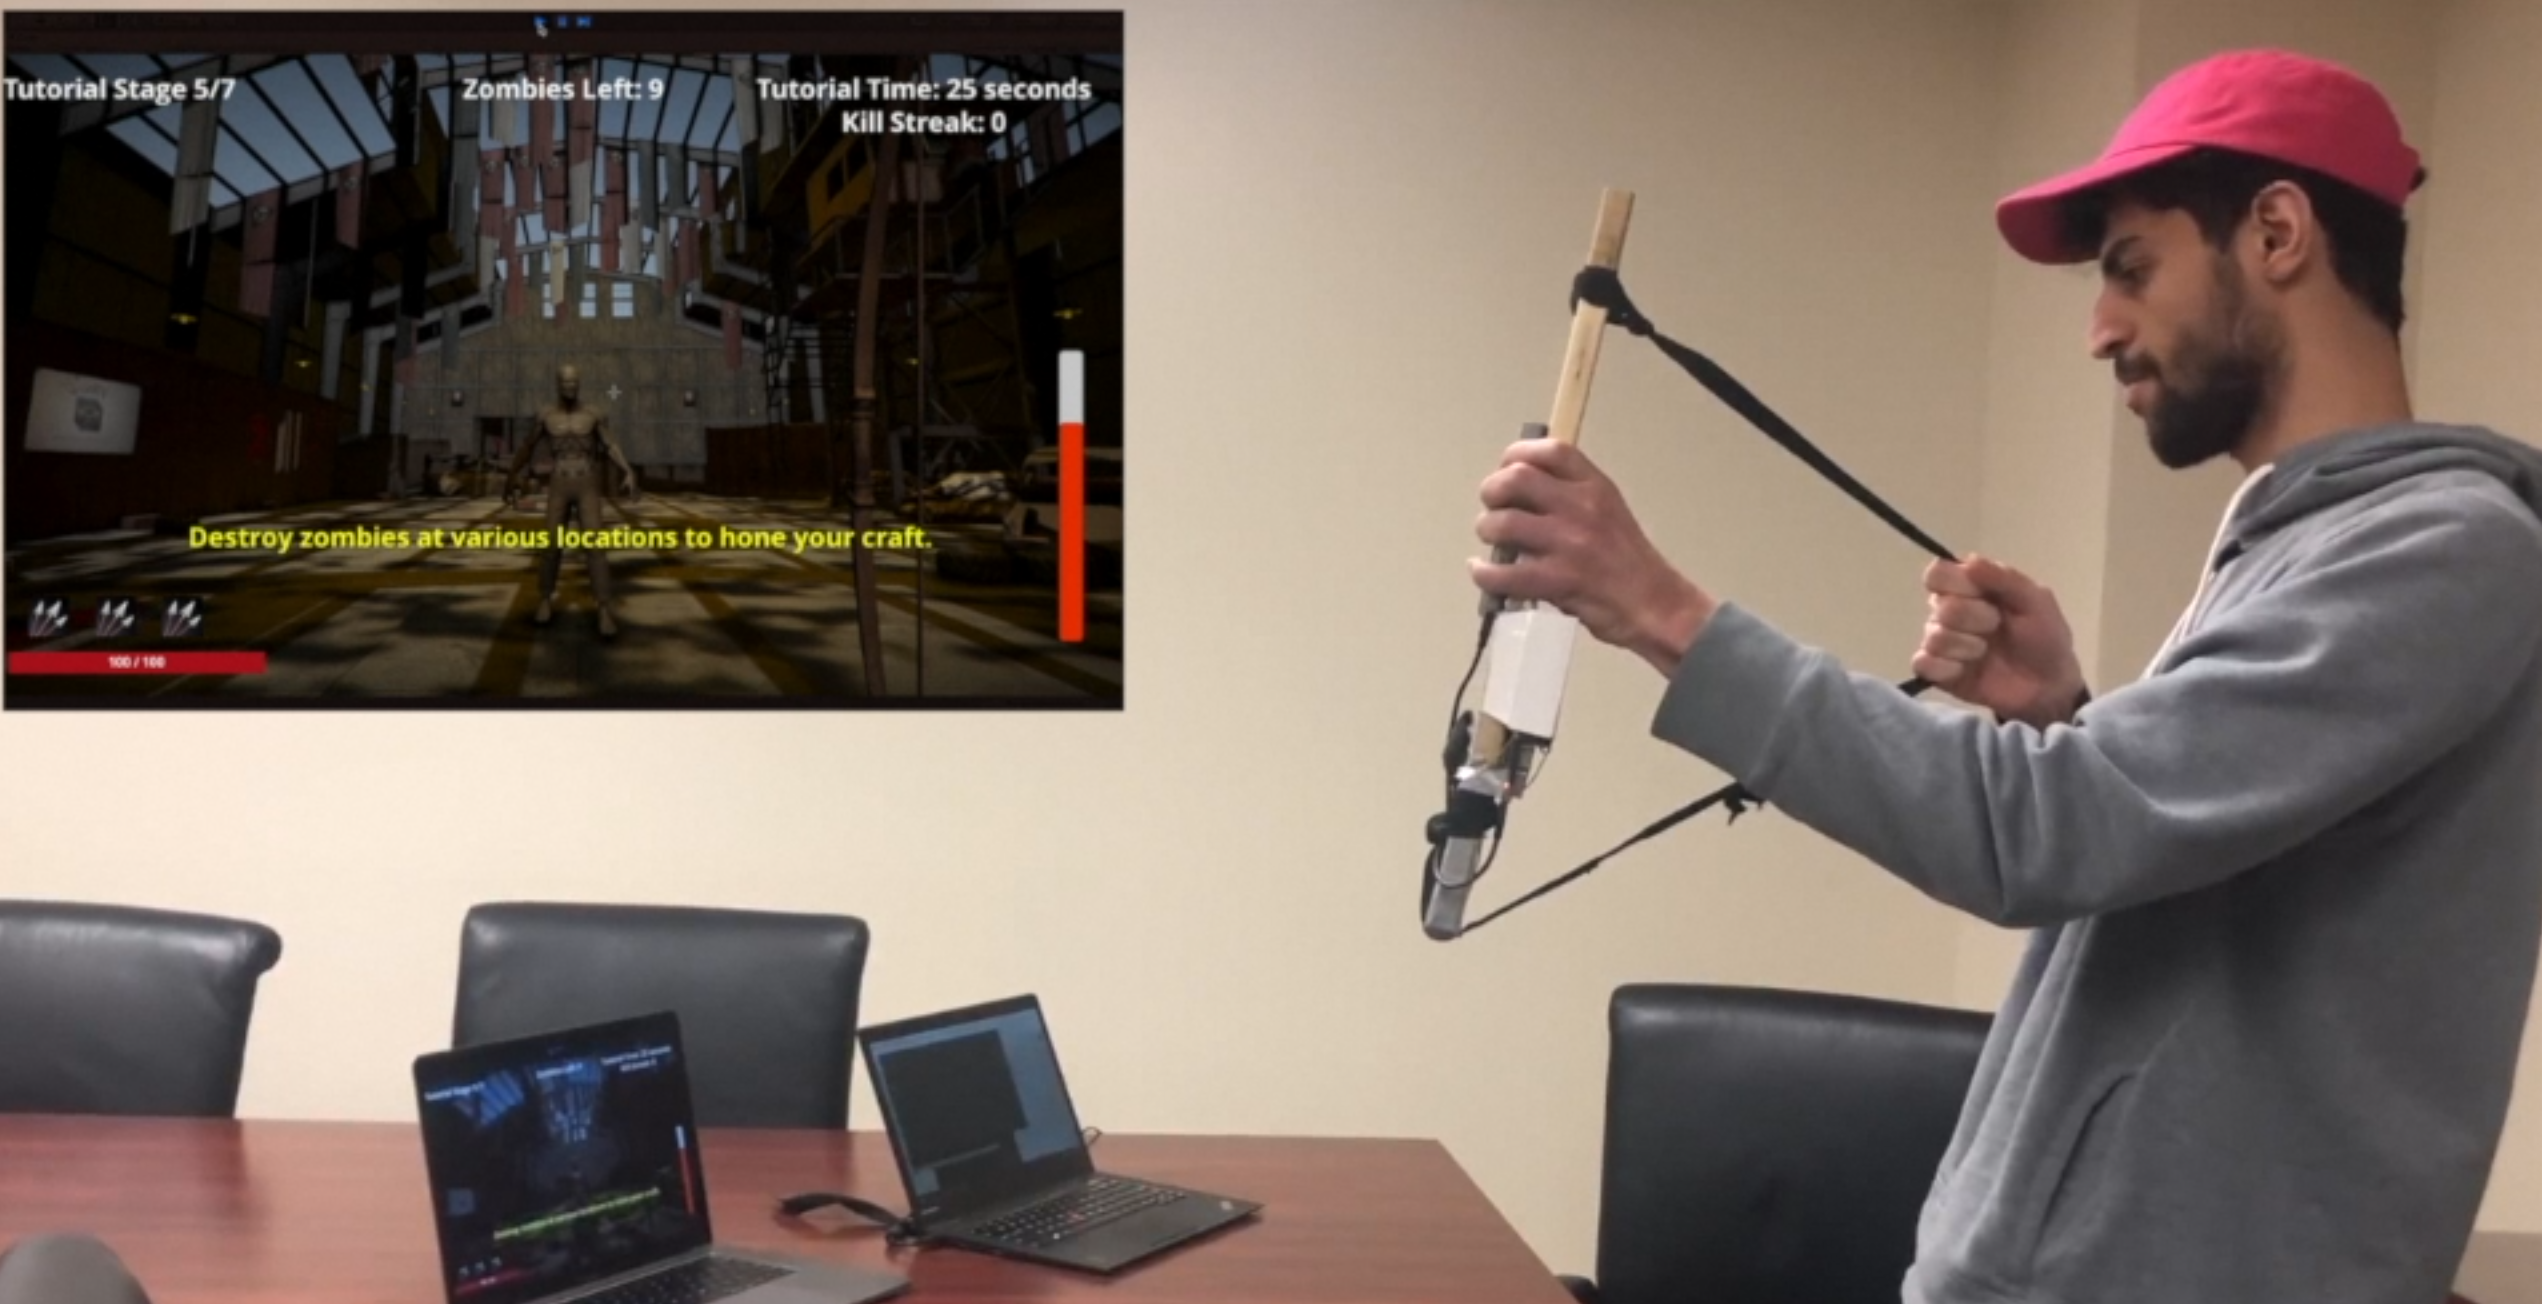
\includegraphics[scale=0.3]{figures/Gameplay_Picture.png}
            \caption{Game-play of ZombieArcher}
            \label{fig:external_shot}
        \end{figure}
        \par
        The game design is inspired by the recent trend in employing new modes of interaction in games and other forms of entertainment. Devices such as Virtual Reality headsets and accurate motion tracking through inertial motion sensors and computer vision allow the user to interact with the virtual world in a more natural way. This idea is explored in ZombieArcher by providing the user with multiple modes of input to the game, such as aiming based on the game controller's orientation, motion gestures that mimic the action of melee and reloading, variable arrow launch force based on the tension in the controller's string, as well as voice commands for in game actions.
    \subsection{Larger Context}
        This game has tremendous potential to be used in other contexts. At its core, ZombieArcher serves to facilitate improvement in hand-eye coordination and peripheral vision. Thus, it has scope to be used in medical applications. Particularly, a modified version of the simulation can serve to provide physical therapy to patients who have suffered physical injury to their arms and torso. Additionally, the game can serve as a mental acuity test to determine the coordination of young children in the context of elementary and middle schools. \par
        Along with medical applications, the game can be modified for military uses. It can serve to prepare soldiers for hands-on training with various weapons and instill safe weapon handling practices. Within this vein, the simulation can be extended to law enforcement and be used in weapon training courses.
\section{Hardware} 
    \subsection{Design}
     The game's controller one of the main hardware components which the player uses to control the character in-game. It is designed to physically resemble a bow and arrow, and is primarily used to aim and shoot the arrow in the game. The user holds the controller and moves it around to aim, and pulls and releases the string to launch the arrow at the desired time and force, in much the same as a real bow. In order to detect the amount of force by which the user is pulling the string, a force sensitive resistor is attached at the bottom of the bow, at the point where the bow string wraps around. As the user pulls the string with increasing force, the tension in the string proportionally applies an upward force where the force sensor is attached. To convert the force sensor's resistance to a digital value, it is part of a voltage divider circuit, as shown in Figure 2. Increasing the force reduces the sensor's resistance, and the circuit is designed to measure the voltage across the constant resistor that is connected to the ground, so increasing the applied force results in an increase in the measured voltage. Since the measured voltage value is an analog signal, and the Raspberry Pi does not contain an integrated analog-to-digital converter (ADC), the MCP3008 ADC chip is used, which converts the sensor circuit's output voltage to a value between 0 and 1023, and communicates the sampled and quantized voltage signal to the Raspberry Pi with the SPI interface. \par
    \begin{figure}
        \centering
        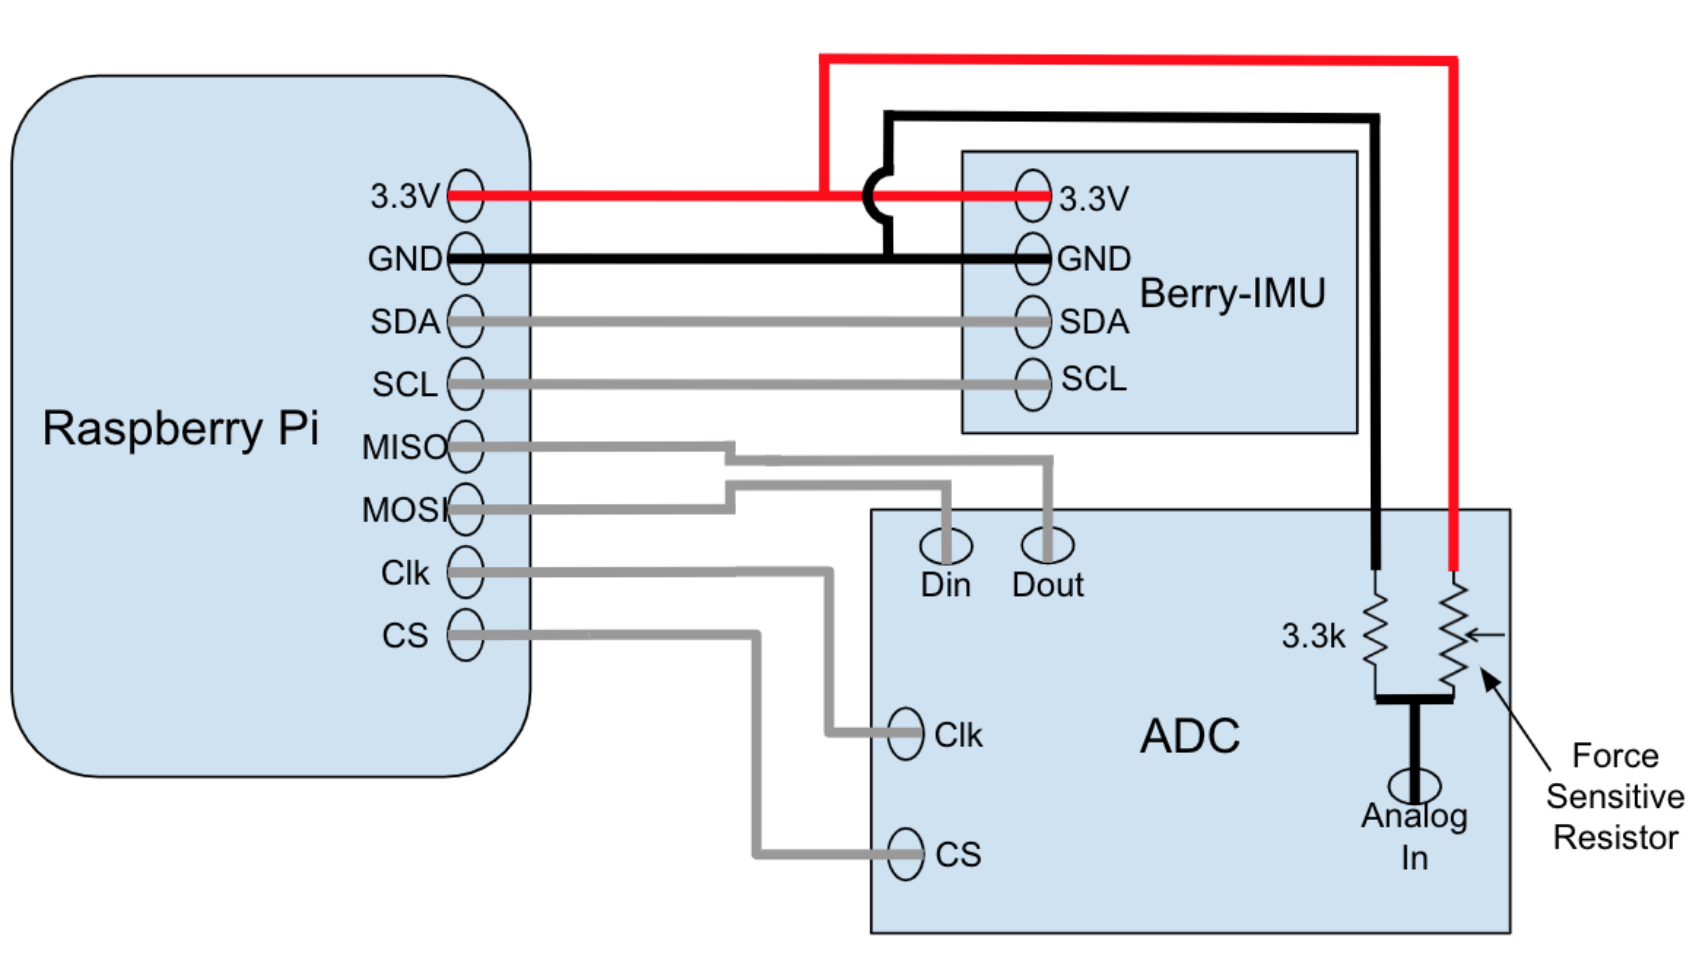
\includegraphics[width=\textwidth]{figures/controller_circuit.png}
        \caption{Wiring layout of the controller's subcomponents}
        \label{fig:circuit}
    \end{figure}
    Although the force sensitive resistor has a linear relationship between its resistance and the applied force in Newtons, the nonlinearities in the measured voltage due to the voltage divider circuit coupled with the nonlinearities in human perception of applied force meant that the raw measured voltage did not feel linearly related with the perceived applied force. In order to fix this, the measured sensor value is limited by a threshold floor and ceiling value, and is mapped to a logarithmic scale in order to give the user a more progressive feel of applied force. \par
   The controller's aiming direction is determined by its orientation in the real world, which is measured using the onboard BerryIMU's accelerometer, gyroscope, and magnetometer. To enable orientation tracking in three dimensions, the Madgwick AHRS algorithm, developed by Sebastian O.H. Madgwick, is used, which uses BerryIMU's sensor readings to calculate the change in the controller's orientation in the form of quaternions. The use of quaternions is advantageous as it allows for uniquely representing all possible orientations of the controller unlike the Euler system. The BerryIMU is also used to detect motion based gestures such as reloading the available arrows and melee. It does so by using the orientation calculated previously to remove the measurement of gravity from the accelerometer's raw measurements, so that the accelerometer values only correspond to the controller's motions. It then uses this data to determine whether, at any point in time, the motion caused by the player matches the predefined characteristics of certain gestures using a state machine for each defined gesture. It looks for peaks in acceleration, the direction of the motion, and the time elapsed between each successive peak to determine whether the motion was a gesture. \par
   Due to the performance constraints of the Madgwick AHRS algorithm, the orientation and gesture detection aspects of the controller's software were written in C, while the UDP communication and the force sensor measurement code was written in Python. To send the controller's data to the machine running the game in Unity, the python script executes the C program and reads its output, and combines it with force sensor data into a JSON package, and sends it to the UDP server. \par
    \subsection{Difficulties Encountered}
    One of the largest challenges throughout the development of the game controller was to minimize the background noise from BerryIMU's raw sensor readings to make the aim accurate enough to allow the player to consistently hit a target in the game without any jitter, and to minimize the long term accumulation error due to integrating the gyroscope readings of the rate of rotation, causing the in game orientation to drift away from the physical controller's orientation. Due to the highly noisy nature of the IMU's readings, several filtering techniques such as setting minimum value thresholds and a sliding average of the past sensor readings were employed. While this did not completely alleviate the issues stemming from the noise in the data, such techniques significantly reduced both types of errors. While this improved the aiming accuracy of the controller, the gyroscopic drift was still large enough to be noticeable after a few minutes of gameplay. \par
    In order to fix such issues, it was necessary to find an external source of measuring orientation that was immune to such long term errors. For this, we used a user facing camera along with OpenCV to measure the lateral location of the controller by tracking the vertical pixels that the controller occupied in the camera's frame of reference. Although this measurement doesn't directly measure the controller's rotation about the Z axis, it gives a drift free approximation which is used as a ballpark to compare to the controller's calculated rotation about the Z axis. Similarly, to get rid of drift in the vertical aim, the accelerometer data was used by calculating the ratio of the component of the gravity affecting the Z axis and the Y axis. Since both the accelerometer based vertical aim and camera based lateral aim contained a large amount of noise, we couldn't directly use them to measure the final orientation. Instead, a proportional feedback loop was used in order adjust the final orientation from the one calculated with the Madgwick algorithm proportionally in the direction of the difference with respect to the externally measured orientation. \par
    \subsection{Experimental Verification}
    Testing and data analysis was crucial in the development process of the controller, in order to refine and polish the feel of the game's controls. In almost all aspects of the game, compromises between certain desired characteristics of the controller were made to ensure the best possible usage experience given the constraints. For the filtering of the raw BerryIMU sensor readings, it was important to get rid of as much background noise as possible without filtering out the useful information. In the case of the gyroscope, for example, setting the minimum value threshold too low would result in rapid accumulation of error in integrating the gyroscope data, while too high of a threshold would alleviate such error but introduce another form of error by not sensing subtle changes in the controller's orientation. Issues such as these were resolved by designing tests that would test a particular shortcoming in the controller software, and through testing the controller in game in multiple scenarios to determine the degree of accuracy and consistency that would be sufficient for our purposes, and which aspects of the controller's functionality were a higher priority to achieve compared to others. For example, by collecting subjective feedback regarding the action of pulling the bow string and launching the bow, we determined that while detecting a large range of forces to launch the bow allows for potentially higher precision in controlling the arrow launch speed, reducing the range of forces allowed for a much more consistent and progressive feeling arrow launches, which were more important for a good gameplay experience than precision. \par
    \begin{figure}
        \centering
        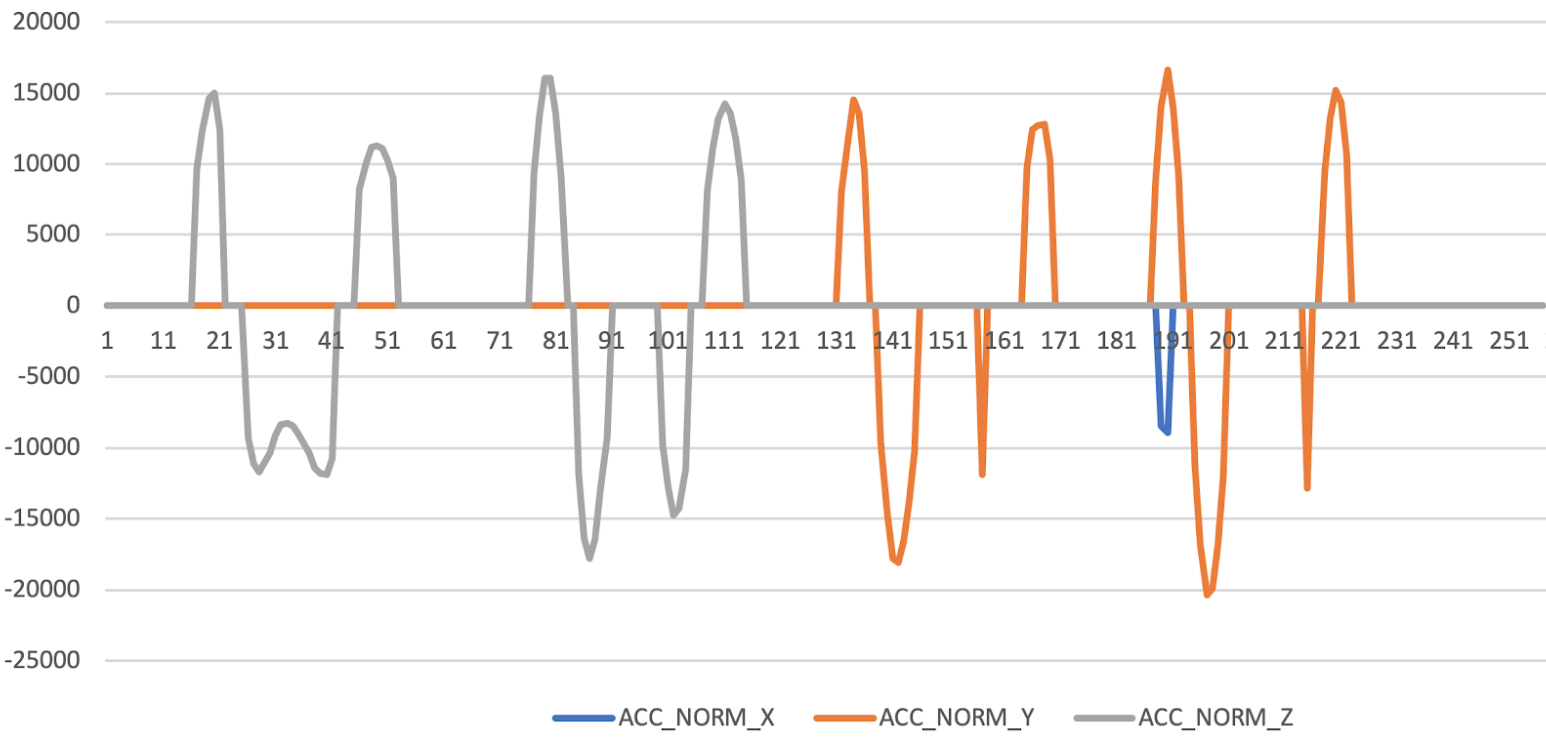
\includegraphics[width=\textwidth]{figures/gestures.png}
        \caption{Accelerometer data for melee and reload gestures}
        \label{fig:gestures}
    \end{figure}
    Experimental testing was also important in choosing the characteristics and features required to detect the motion based gestures of melee and reloading. Since every player will have a slightly different way of holding the controller and performing the gesture, we first collected IMU telemetry for over fifty different instances of the gesture that were deemed correct, some of which are shown in Figure 3, as well as several instances of incorrect gestures. By analyzing the range of speeds and magnitudes of the various correct gestures, the most common features were the number of peaks in the acceleration, the difference in the highest and the lowest peaks, and the range of time elapsed between each peak. This information was used to define the parameters that the state machine would look for when detecting a gesture. \par
\section{Image Processing}
    \subsection{Design}
    The game employed one laptop camera that detected color, quadrant, and column. In order to play the game, the player was required to wear a bright pink hat to be detected by the camera. The purpose of this was for the camera to easily distinguish between the player's location and the background colors. When the player was within an acceptable range, the camera would easily detect the pink and tell the game to resume operation. In addition, a second player was required to wear a bright green glove to enable the adversarial multiplayer mode. In this multiplayer mode, the second player would continuously hold up the glove to the camera for a few seconds and once detected, the camera would tell the game to spawn a zombie for the first player to kill. The camera also had quadrant detection for the glove and whichever quadrant the glove was held at corresponded to the spawn location of the zombie. For example, if the glove was held at the upper right hand quadrant, the game would spawn a zombie in the far right of the map. Lastly, the camera detected which column of the frame the bow was in to help reduce the gyroscopic drift. If the gyroscope ever strayed away from its original column, it would return to its originally detected column.\par
    The image processing was implemented in Python using the OpenCV package and was largely based off of the work of \cite{Mordvintsev_2013} and \cite{Sharma}. The program first opened up the camera and analyzed the video frame by frame. From there, each frame was converted to a HSV (Hue Saturation Value) image as it is easier to analyze with this color scheme than in RGB (Red Green Blue). Then the HSV image was thresholded to create a mask which kept only the color we wanted and made the rest of the frame black. Finally, the mask was bitwise-ANDed with the original image to keep only the color in the frame we wanted and filter out everything else. After the frame had been filtered, a blur was applied to smooth out the image and reduce background noise. This was to stabilize the image, making it easier for the camera to detect the pertinent object and prevent the camera from detecting any extraneous objects or light that might have been in the background. After the blur was applied, the camera found the contours of the image and drew a contour around it to track the object. For the column detection, the camera also found the centroid of the object and drew two vertical lines of equal distance to the left and right of it. For the quadrant detection, the camera divided up the frame into four quadrants, found the centroid of the object, and checked which quadrant the object was in.
    \begin{figure}[ht!]
        \centering
        \begin{subfigure}[b]{0.4\linewidth}
            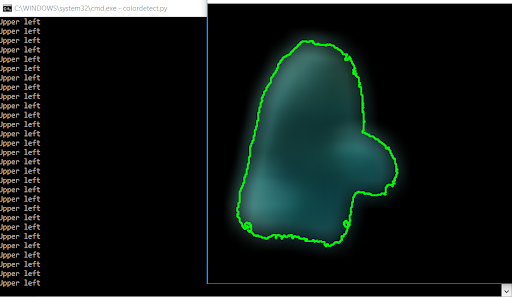
\includegraphics[width=\textwidth]{figures/glove.png}
            \caption{The detected glove and quadrant}
        \end{subfigure}
        \begin{subfigure}[b]{0.4\linewidth}
            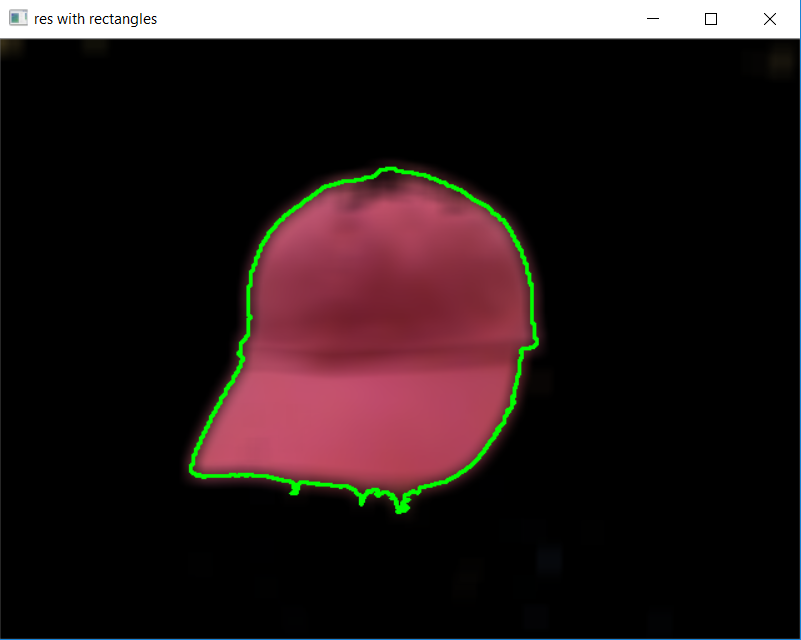
\includegraphics[width=\linewidth]{figures/hat.png}
            \caption{The detected hat}
        \end{subfigure}
        \begin{subfigure}[b]{0.4\linewidth}
            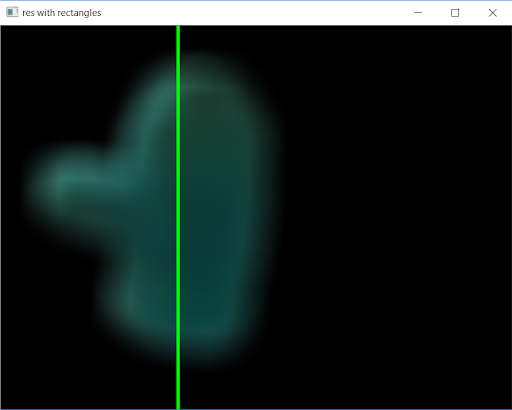
\includegraphics[width=\linewidth]{figures/column.png}
            \caption{Column detection with the hat. In the game, it was applied to the bow.}
        \end{subfigure}
    \end{figure}
    
    \subsection{Difficulties Encountered}
    The first difficulty encountered was finding acceptable threshold ranges for the object detection; appropriate ranges must be chosen for both the color filtering and the blur. For the color threshold range, if the range was too wide, then too much color would be picked up and the camera would not be able to distinguish between the desired object and the background. If the range was too narrow, then too much color would be filtered out and the camera would not detect anything at all. For the blurring, if the kernel dimension was too small, then there would be too little blurring which would make it hard for the camera to detect the whole object. On the other hand, if the kernel dimension was too large, then the desired object would be blurred too much and almost fade away into the background. I had to experiment with the ranges until I found one that was acceptable. \par
    In addition to finding acceptable threshold ranges, we had to ensure that the camera detected the quadrants correctly. At first, the object would behave strangely around the edges of the quadrants due to the camera detecting the top left edge of the object, so we switched to centroid detection instead for more robust detection. In addition, we had to make sure that the camera would stop detecting once the object moved outside of the screen, so we ensured that detection was done only when the object was present.
    Lastly, I had to refine the column size until I found one that reduced the gyroscopic drift smoothly. If the columns were too wide the gyroscope would move too slowly and if they were too narrow the gyroscope movement would be too jerky.
    \subsection{Experimental Verification}
    I tested out the object detection with different lighting levels, different background colors, and movement. I did this to ensure that the object detection was robust and would work in a variety of different environments. I varied the lighting conditions, background colors, and had the players move and then ran the game to see if it would work properly. I modified the threshold values until the game worked properly under those different conditions.\par
    Similarly, I tested the quadrant detection by having the player hold the glove in each quadrant and seeing if the game spawned a zombie in the correct quadrant. I also made sure that this worked with different lighting levels, different background colors, and with glove movement.\par
    Lastly, I tested out the column detection by varying the column size and seeing which size best reduced the gyroscopic drift while ensuring smooth movement. I modified the column size and played he game to see which size resulted in the smoothest gameplay.
   

\section{Speech Processing}
    \subsection{Design}
        \begin{figure}
            \centering
            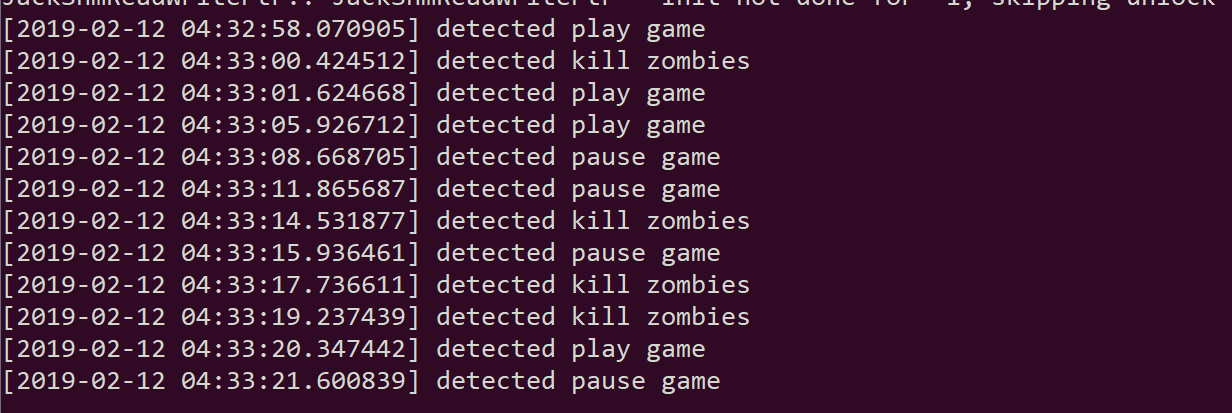
\includegraphics{figures/speech_recognition.PNG}
            \caption{Terminal output showing the Porcupine library’s detection capabilities for trained hotwords.}
            \label{fig:speech_recognition}
        \end{figure}
        The speech recognition and processing portion of the ZombieArcher game was finished this quarter. We chose the Picovoice Porcupine library to detect so-called "wake-words". When a player uses the phrases "play game", "pause game", "kill zombies", or "show statistics" the game responds by performing the associated control actions. As expected, the "play game" and "pause game" commands start and stop the game, respectively. The "kill zombies" command instantiates a power-up, which is only available after the player has successfully killed three zombies. Additionally, the "show statistics" command displays the player's shot statistics and rank on the screen for five seconds. \par
        In order to implement all of these wake-words with the Porcupine library implementation, we had to train models for each of the phrases. To do this, we used the library's optimizer tool to provide hundreds of pieces of ground truth. More specifically, we recorded ourselves and various speakers saying the phrases repeatedly and in varying ambient noise conditions. After we developed the models for all four keywords, we passed the generated files to a speech detection class in the library and were able to detect all utterances of the phrases in a non-blocking manner. This allows the game to continue on even if there is no speech input from the player. \par
    \subsection{Difficulties Encountered}
        The speech processing part of the game was rife with difficulties. However, we were able to overcome all of them. First of all, we had decided to use the Google Speech-to-Text API as suggested by many of our peers. In order to implement it though, we needed a linux machine with proper python programming facilities and access to attached hardware devices \cite{ishant_2013}. As none of our team had one readily available, we decided to instantiate a virtual machine. After doing this, we were forced to spend time collecting the necessary packages and drivers required for our test machine to be able to use the internal microphone for speech collection. \par
        Upon solving the virtual machine issue, our game ran fine with the Google API. However, we soon realized that the Google Speech-to-Text implementation introduced substantial latency into the system. This is because the program had to first collect speech input from the player, then, we sent the data to Google's systems. Finally, after Google's analysis, we received the final result and parsed it. This system was extremely processor and time intensive, which was not acceptable for a real-time game implementation. To combat this issue, we decided to use the Porcupine library. \par
        The Porcupine library proved to be the solution we were looking for. After the labor intensive neural network model training, we had a hot-word detection system that could use our custom phrases and detect utterances with a very high confidence level. \par
        A final issue we ran into was with the licensing for the Porcupine library. It turned out that each of the custom keywords were only usable in a non-commercial context without a full license. This was completely fine for our purposes. Despite this, we found that the keywords we generated would quickly expire after a few days and would prevent the program from running. After contacting the library's creator, he provided me with a custom optimizer tool, which would allow for the generated keywords to last up to 75 days. Thus, we were able to solve all of our issues and successfully complete the speech collection and recognition part of the ZombieArcher game. \par
    \subsection{Experimental Verification}
        After training the appropriate models, we tested the hotword detection capability in numerous environments (quiet, moderate, and loud) and with different people. We have found that using the neural-network based approach, the success rate of keyword detection is much higher than with a Speech to Text transcription API, such as Google’s. Furthermore, during our research, we learned that a similar hot word detection approach is used in Amazon’s Alexa and Apple’s Siri platforms. \par
        We found an overall detection success rate of 81.48\% and a success rate of 100\% in quiet conditions. Additionally, over a span of five different speakers, there was a success rate of roughly 75\%-85\% in the three environments. As we made our measurements with the internal microphone present on a laptop, we believe the success rate will increase substantially with an external microphone. Additionally, we expect that players will use the game in a quiet to moderate environment; thus, even though we accounted for loud ambient noise in our testing, these conditions are not optimal.
\section{Unity Game}
    \subsection{Design}
    ZombieArcher offers three modes of gameplay: a tutorial mode, survival mode, and multi-player mode. The tutorial mode is designed to teach the player the necessary skills to succeed in our game. In particular, the tutorial mode teaches the player how to aim and shoot arrows, reload his quiver, perform melee, and utilize power-ups with speech commands. Each stage within the tutorial teaches the player one of these actions by demonstrating how to perform the action with an instructional video. Then, it requires the player to perform the action three times in order to advance. After the player finishes the stages that teach the player important skills, the player is given an opportunity to shoot zombies at varying distances. Figure \ref{fig:tutorial} shows the layout of the first stage of the tutorial mode. The tutorial mode also allows the player to learn the tools available to him in the user interface. For instance, the player can see his current health, number of arrows in his quiver, and the force he is applying to the arrow in real time. 
        \begin{figure}
            \centering
            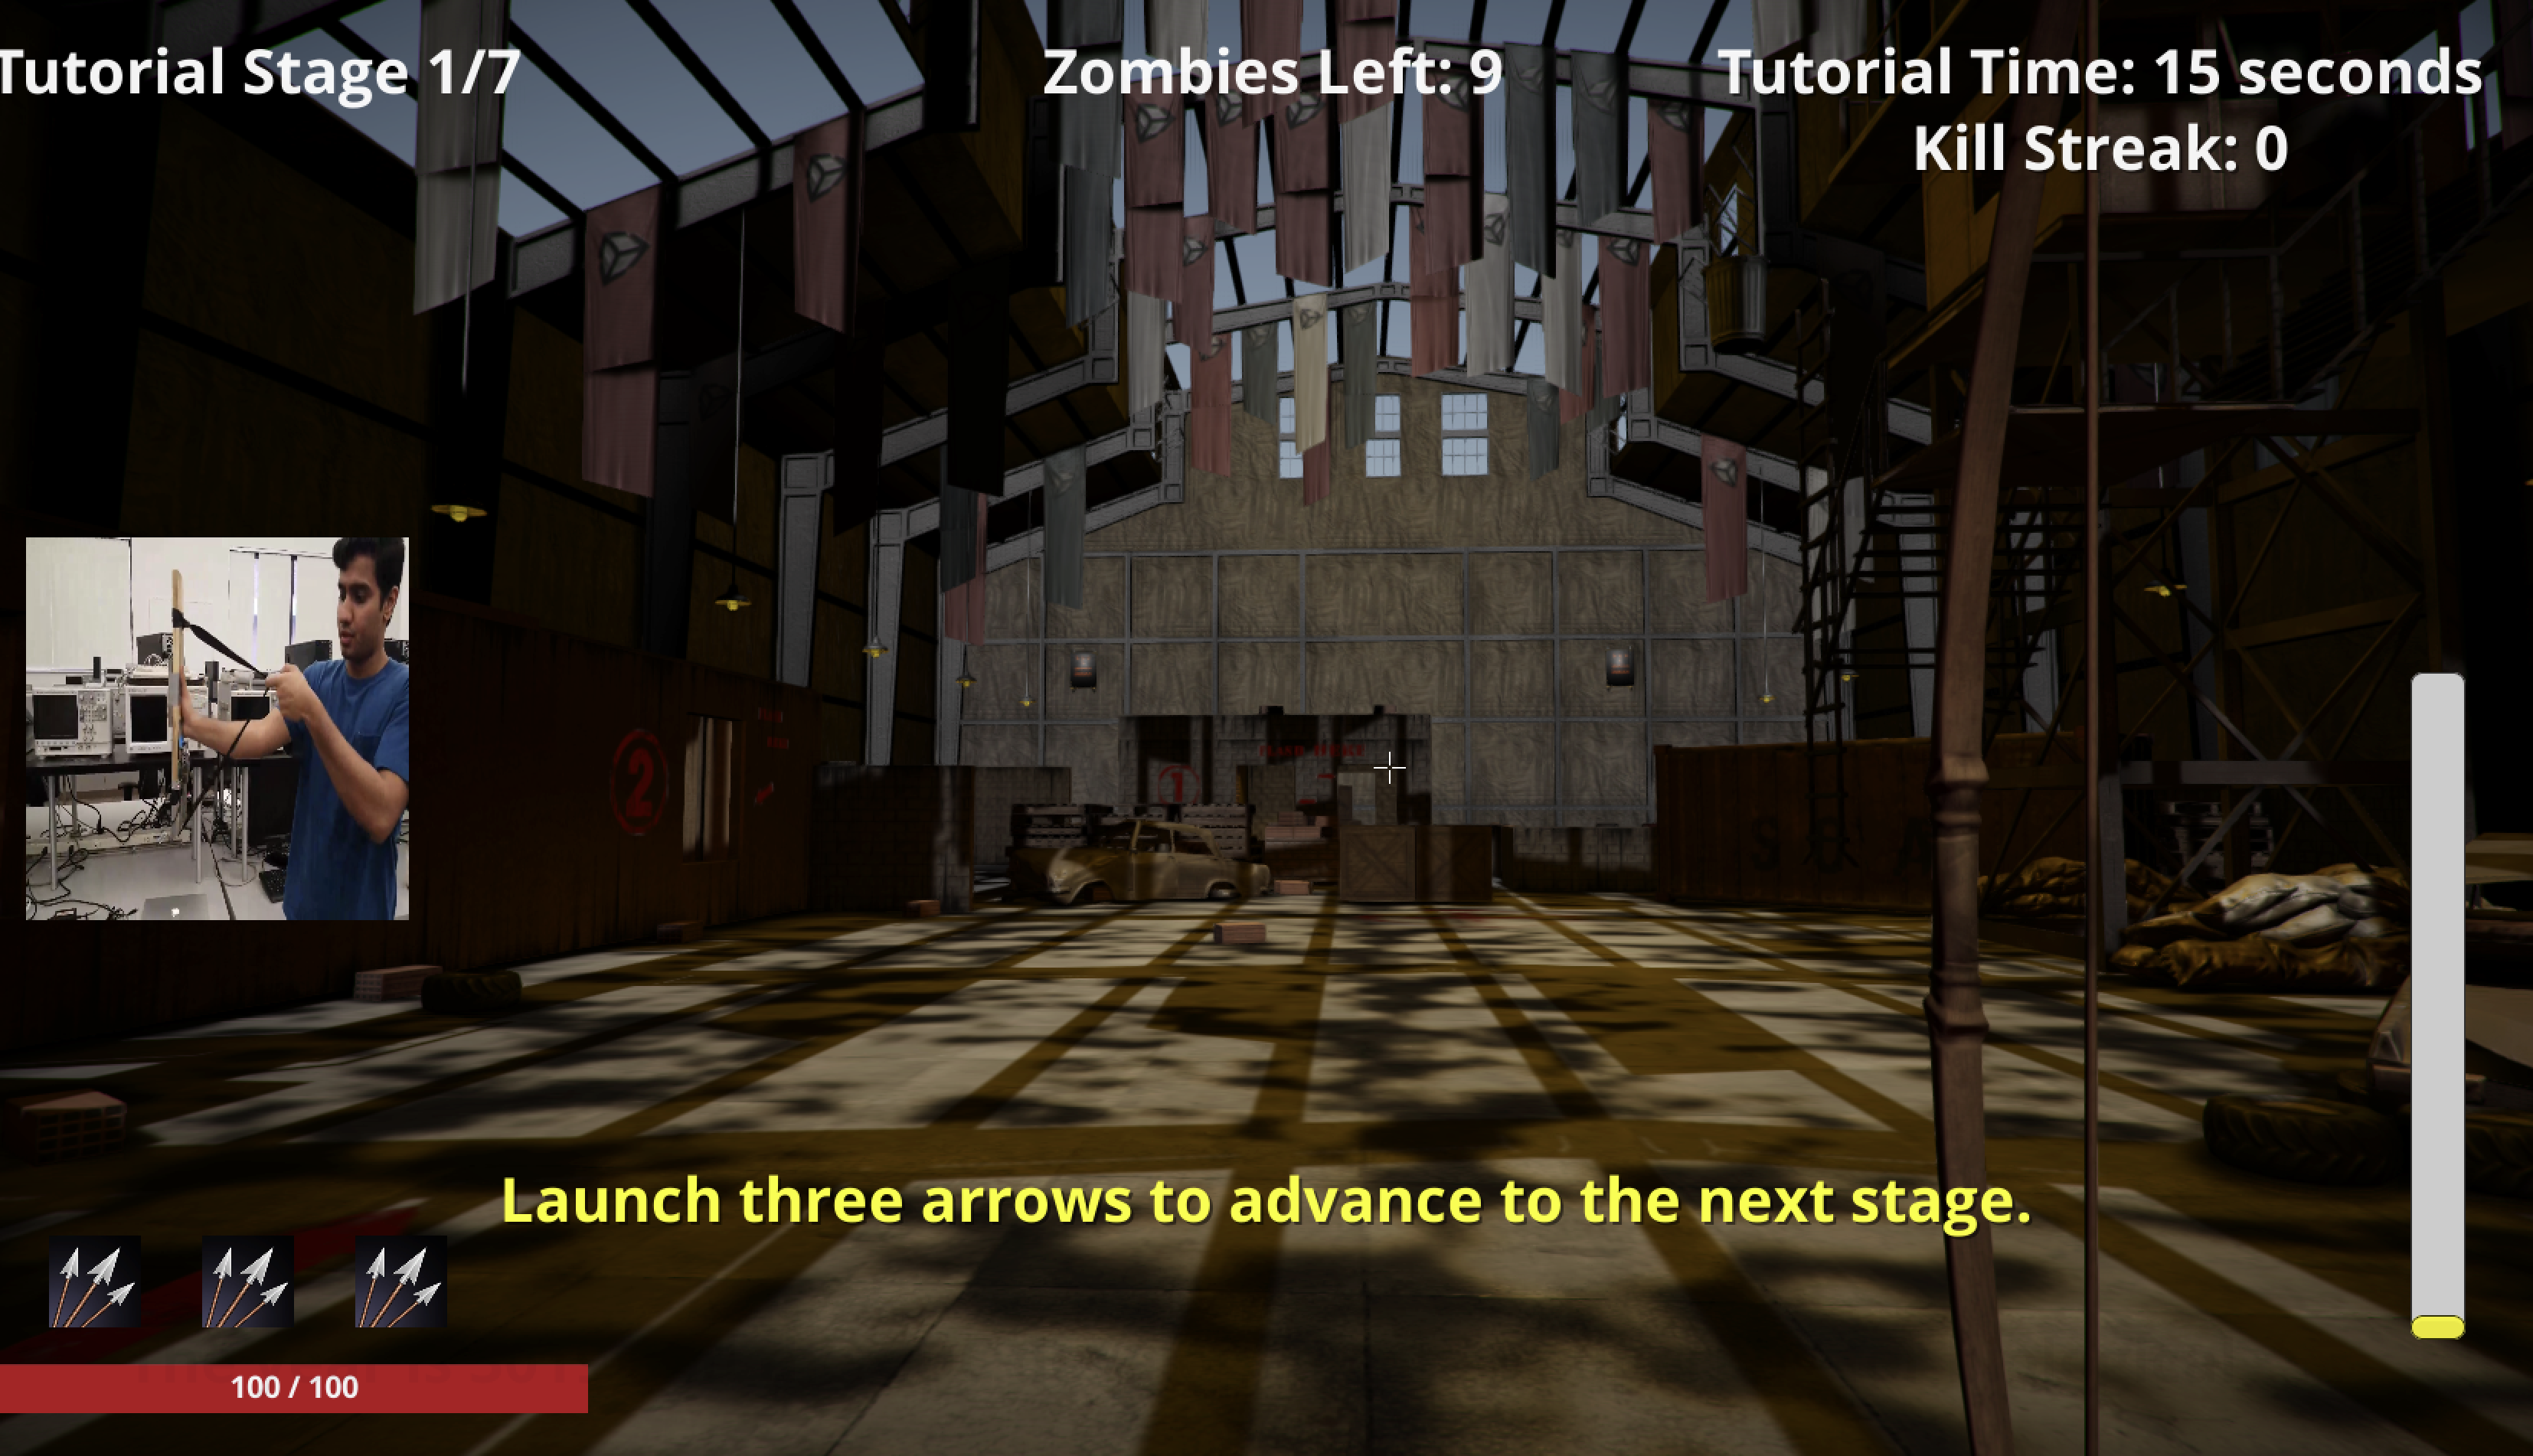
\includegraphics[scale=0.3]{figures/tutorial.png}
            \caption{Stage 1 Layout for Tutorial Mode.}
            \label{fig:tutorial}
        \end{figure}
    \par
    The goal for the player in the survival mode is to stay alive as long as possible by destroying zombies with arrows, melee, and nuke power-ups. Meanwhile, the game controller adjusts to the player's skill level by changing the speed of the zombies, spawn frequency, and number of active zombies. Furthermore, if the player is performing poorly, the game controller may decide that the player needs to replay the tutorial stage. As an incentive for the player to continually improve his skills, the player unlocks a nuke power-up after every three zombie kills and can store up to three power-ups. By saying the phrase "kill zombies", the player can kill all zombies at once with a nuke. An example of gameplay in the survival mode is shown in Figure \ref{fig:survival}. It shows an example of gameplay where the player is performing quite well. The player successfully destroyed six zombies and has unlocked two nukes. Initially, only two zombies can be in the scene at a given time; however, the game controller has decided to allow more zombies on the scene based on the player's performance. 
            \begin{figure}
            \centering
            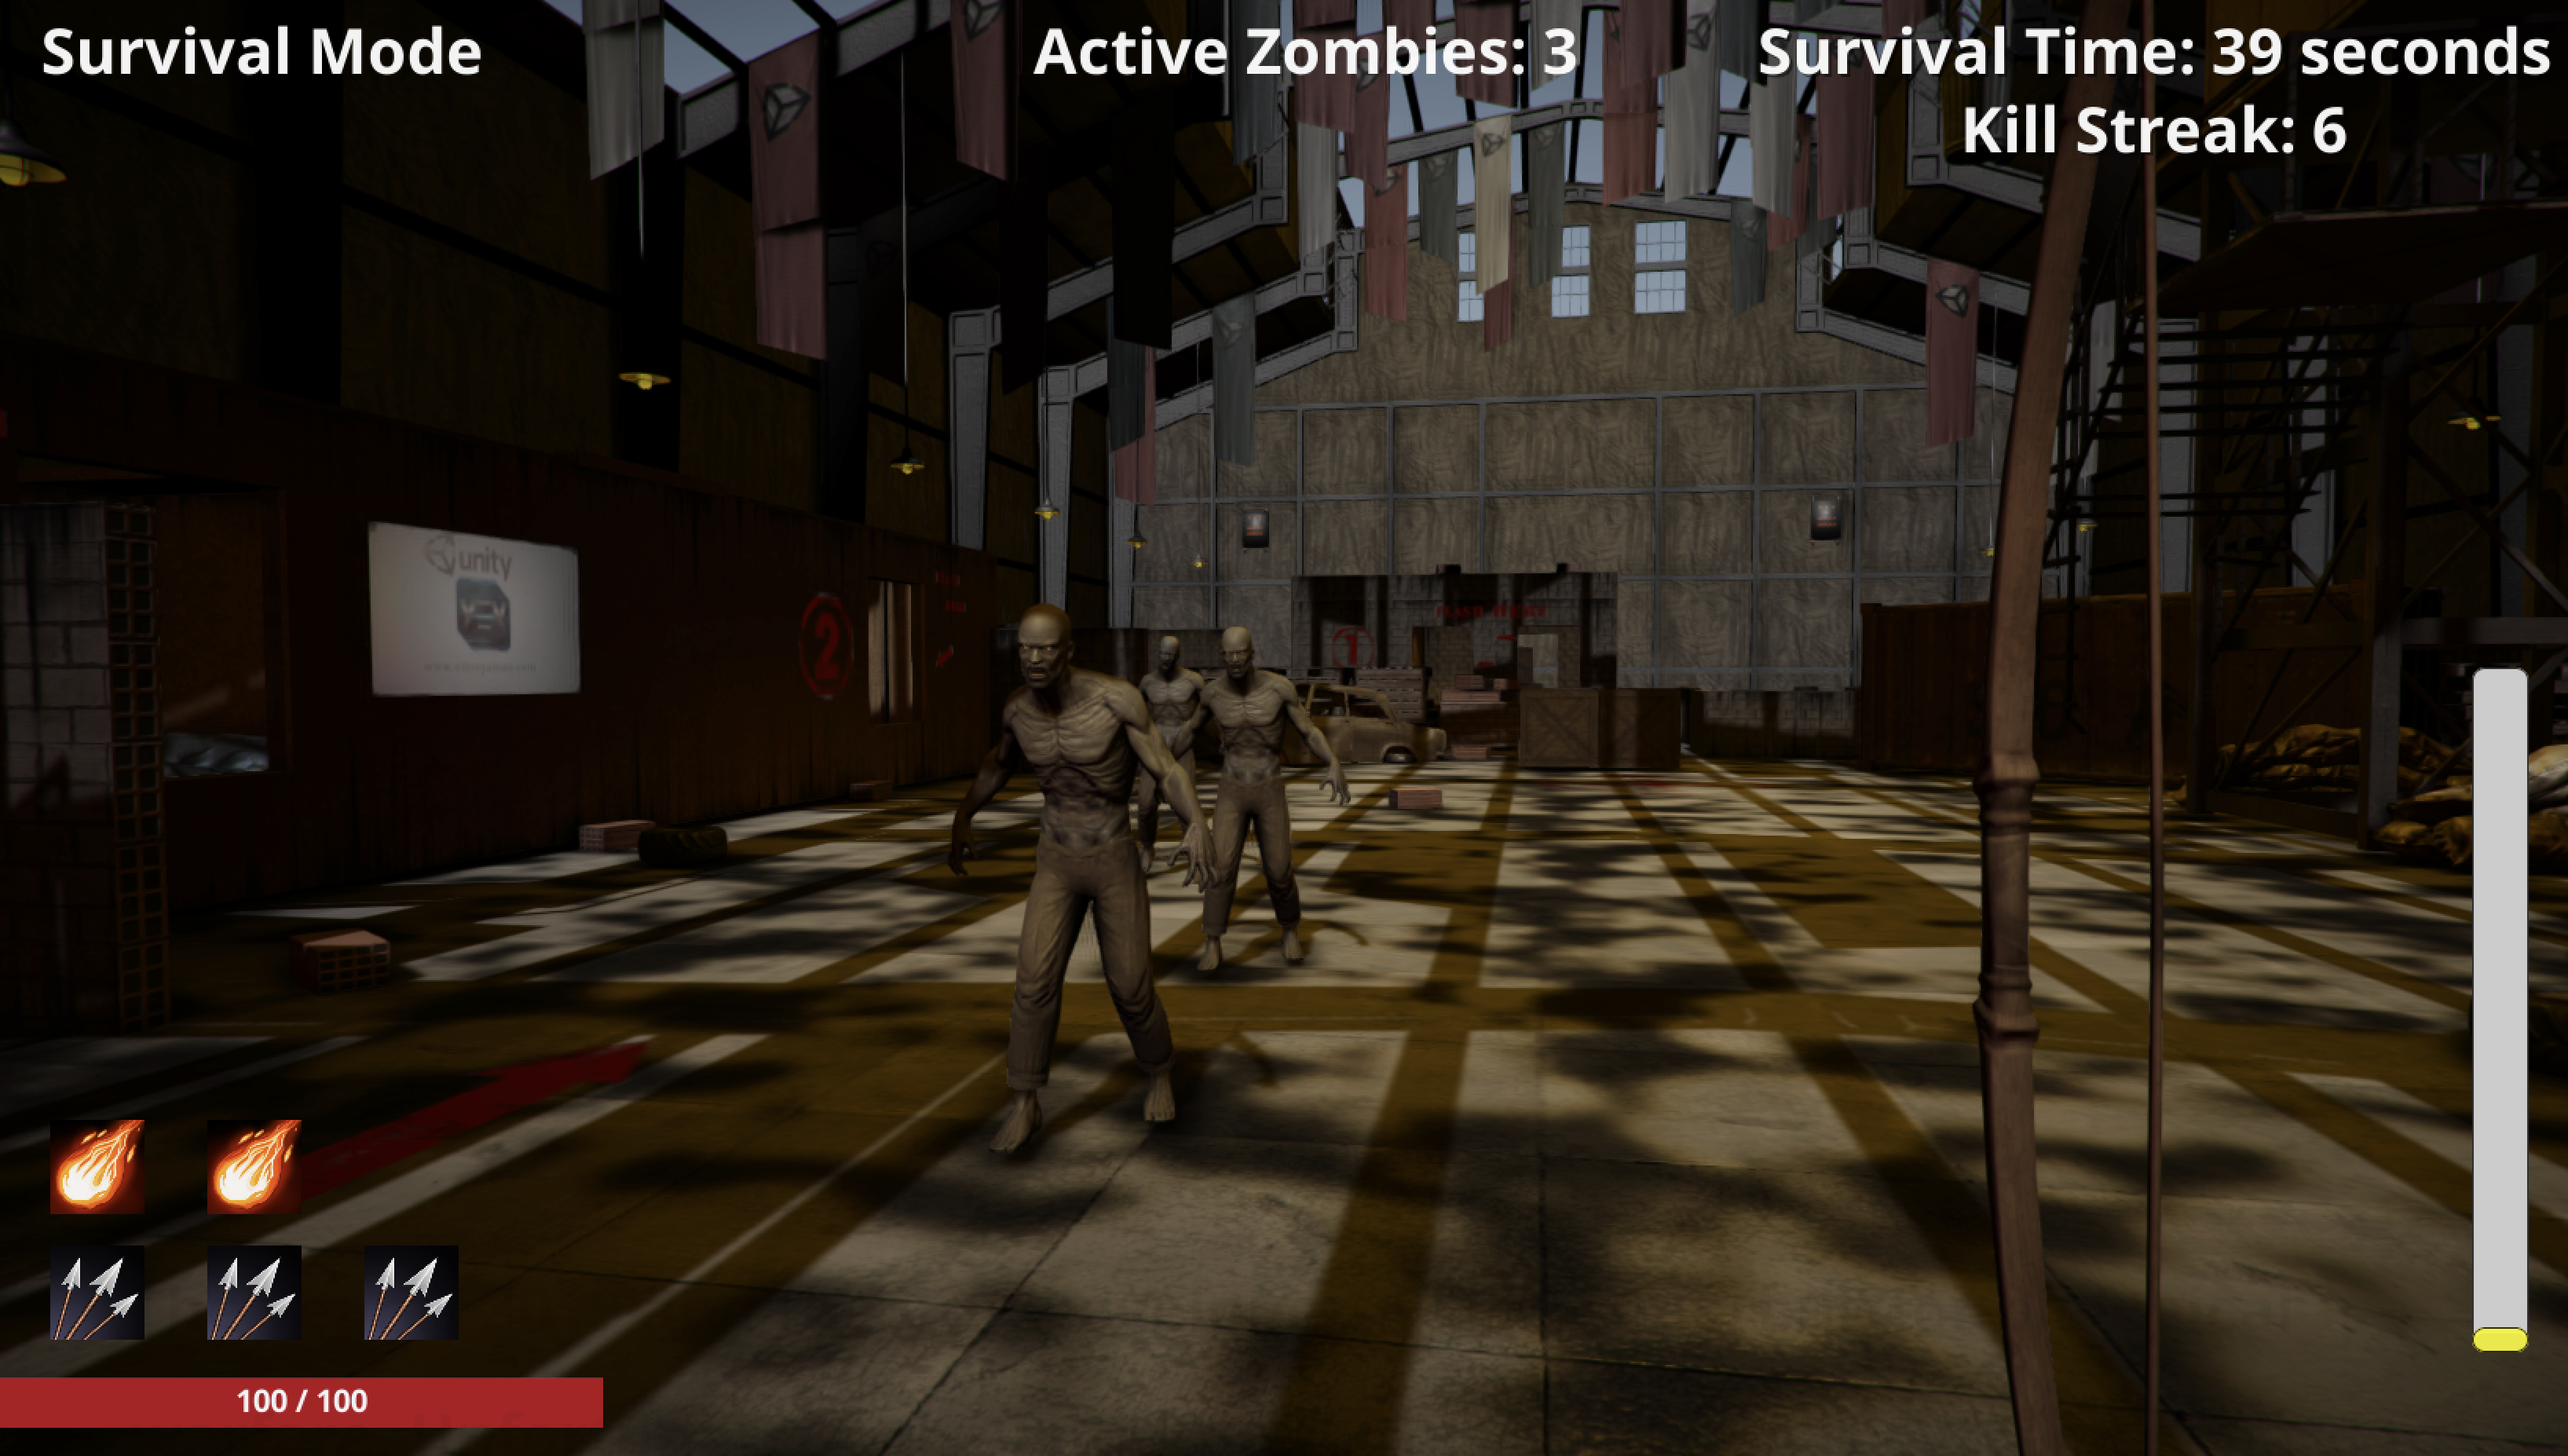
\includegraphics[scale=0.3]{figures/survival.png}
            \caption{Survival Mode Gameplay.}
            \label{fig:survival}
        \end{figure}
    \par
    The multi-player mode allows a second player to choose where to spawn zombies, while the first player kills zombies with arrows and melee. The second player can choose to spawn zombies in four locations by placing a glove in a particular quadrant within the camera's field of view. 

    \subsection{Difficulties Encountered}
    At the start of this project, the primary difficulty was the learning curve associated with C\# programming in Unity. Nonetheless, the abundance of tutorials on C\# programming and the work flow of Unity projects found online alleviated this. After creating the framework of the tutorial and survival modes, it became apparent that managing a large software project was the bigger issue. As new features were introduced later on in the project such as power-ups or melee, bugs would be introduced as a result of assumptions made in the initial framework. This required previous code to be rewritten and generalized to allow for new features. 

    \subsection{Experimental Verification}
    The game dynamics were tested substantially with a keyboard and mouse by playing through each of the modes. The gestures, speech commands, and spawn locations for the multi-player mode were mapped to specific keys. This allowed one to verify the correctness of the game logic without introducing bugs from integrating the hardware. Although using a keyboard and mouse was very useful in testing and debugging basic issues in gameplay, the final testing of gameplay was performed by our partner group with the hardware connected. Our partner group often put themselves into situations not simulated with the keyboard and mouse, revealing small errors in our design. 
    
    \section{Machine/Iterative Learning}
    \subsection{Design}
    The ZombieArcher simulation game requires machine and iterative learning to train the player to successfully shoot zombies at varying speeds, depths, and spawn locations. After the tutorial stage where the player learns the basic mechanics of the game, the player enters a survival mode with the intent to survive as long as possible. Here, the zombies become progressively more difficult and the player is forced to improve his skills. 
    \par
    Before any machine learning could be implemented, we decided to store a bevy of statistics for each player allowing the game to make dynamic decisions. Each player has a user account within the game and the total number of shots, headshots, body shots, and missed shots are stored. Using these parameters, the simulation derives the missed shot percentage, head shot percentage, and body shot percentage.
	\par
	The player’s statistics are stored in a SQL database. For this purpose, we chose to use the SQLite library as it is the most useful for embedded IoT applications due to the database being stored onboard. Thus, we do not need to connect to an external database over the Internet and introduce more latency into the game. Figure \ref{fig:database_structure} shows the tabular structure of the values stored within the database for each player.
	
    \begin{figure}
        \centering
        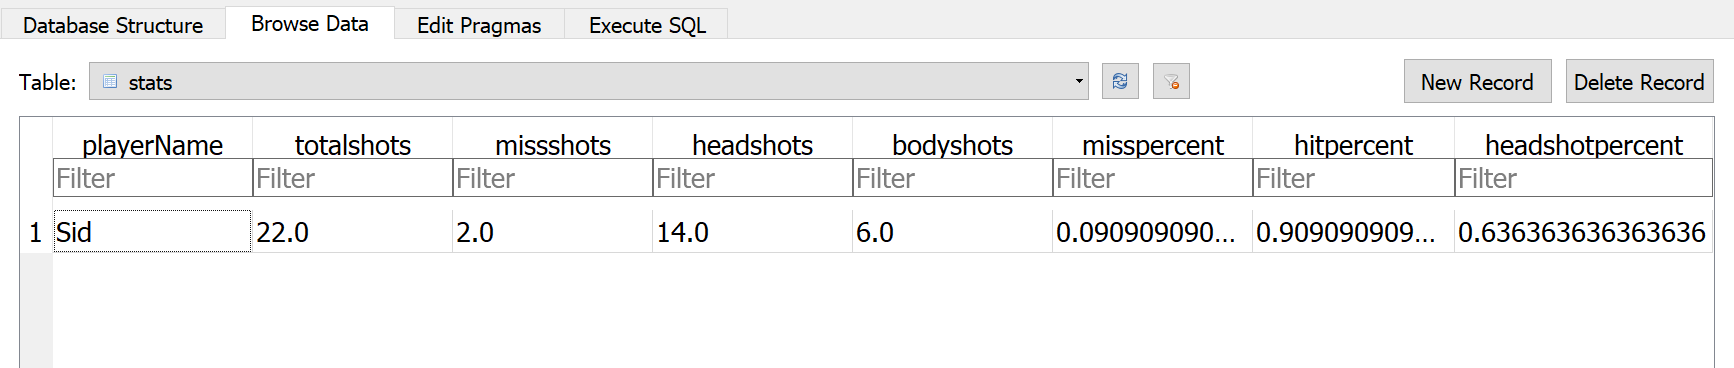
\includegraphics[width=\linewidth]{figures/database_structure.PNG}
            \caption{Structure of SQLite database. The table shows one entry for the user “Sid” along with the associated player statistics and parameters that will be used to make machine learning decisions.}
        \label{fig:database_structure}
    \end{figure}
    
    In order to measure the player’s skill level, a decision tree is used with the player’s hit percentage, head shot percentage, and average reload time as features. The decision tree classifies the player’s skill level into four categories: novice, amateur, advanced, and sharpshooter. The game reacts to the player's skill level by varying dynamics of the game. For instance, when the player is classified as a sharpshooter, the game increases the speed of the zombies, increases the spawn frequency, allows more zombies to be in the scene, and removes the force bar and crosshair from the user interface. The aim of these changes is to ensure that the player is constantly improving and being challenged. 
    
    \subsection{Difficulties Encountered}
    The main difficulty in the machine/iterative learning part of the game was choosing features in the game that adequately measure hand-eye coordination. Our initial approach was to measure was the player's ability to shoot in different directions and distances. However, as multiple zombies can be on the screen at the same time, it was difficult to decide which zombie the player was trying to hit without making erroneous assumptions. As a result, we decided on a more direct approach by simply measuring the player's body hit percentage, head shot percentage, and average reload time. 
    
    \subsection{Experimental Verification}
     The most meaningful testing of the machine/iterative learning portion of the game came from our partner group playing through our game. Our partner group offered us feedback to how well the tutorial teaches the player basic skills, and how the game dynamics change after several minutes of gameplay. We were able to adjust various thresholds of our decision tree to ensure the game remains a fun and challenging experience, regardless of the player's skill level. 
     
\section{Integration}
    \subsection{Design}
        \begin{figure}
        \centering
        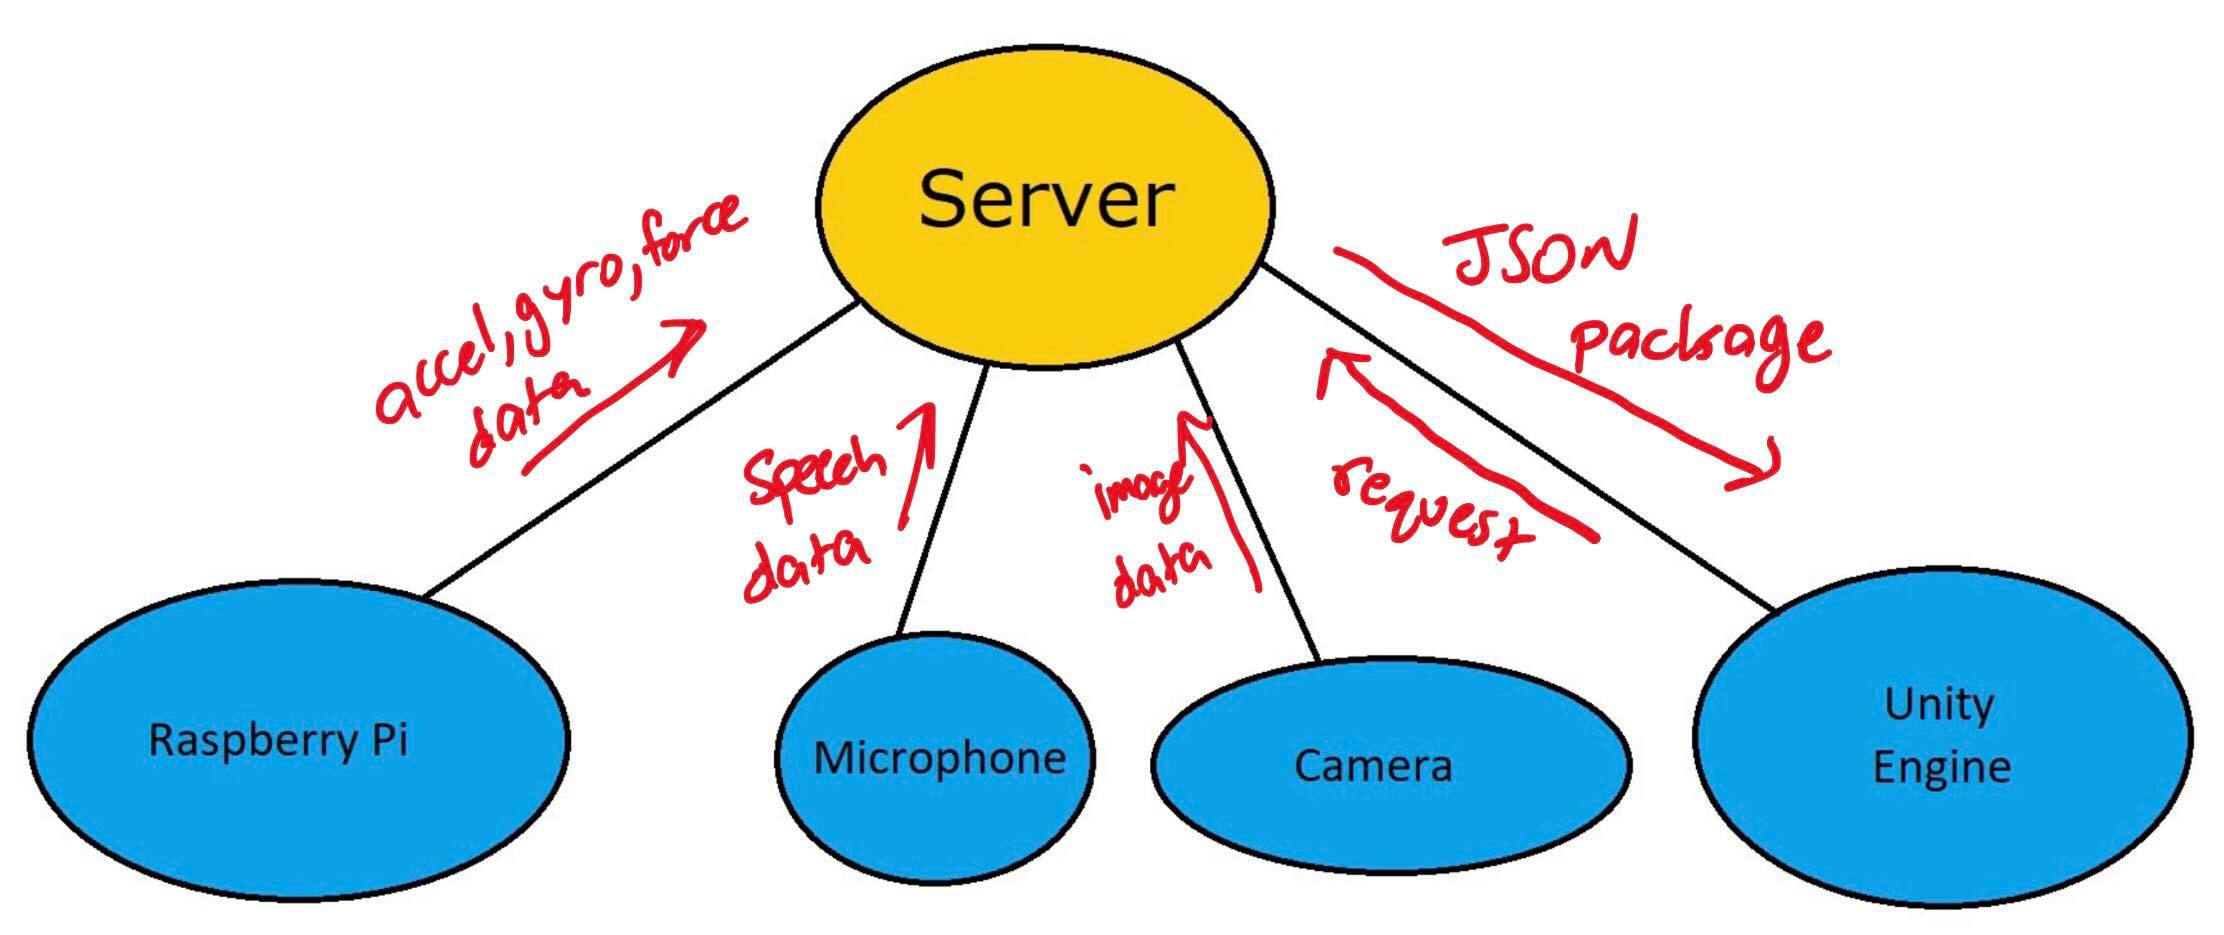
\includegraphics[scale=0.2]{figures/flow_chart.jpg}
        \caption{Process Flow Diagram. Depicts the movement of data throughout the game-play process.}
        \label{fig:flow_chart}
    \end{figure}
        This game's wireless communication system is built on a three-pronged structure. The Raspberry Pi is responsible for the hardware communication. An external laptop runs the simulation under the Unity game engine. A second laptop ties both of these components together as a centralized server.
        Both the server and Raspberry Pi's software are written in Python. They rely heavily on UDP sockets to communicate. While the Unity game is primarily written in C\#, it too depends on UDP sockets for communication. The flow diagram given in Figure \ref{fig:flow_chart} shows the movement of data throughout the game. As of this writing, the game successfully implements communication to all peripheral hardware components.
    \subsection{Difficulties Encountered}
        The greatest difficulty in the integration portion was connecting all of the hardware pieces without code breaking. It seemed that as soon as we added a piece to the larger system it would stop working. To combat this, we set aside time to work when all four of us were available and found that, in most cases, only small modifications were necessary to incorporate the subsystem into the larger game.
    \subsection{Experimental Verification}
        In order to test the integration of the various components, we verified that the data sent to the server was correctly packaged into a JSON object by displaying the object's fields in a console. While the console was displaying the data, stimulus was provided to each of our sensors and we examined whether the data displayed corresponds to the data expected as a result of the stimulus. If the data showed on the console for a particular server was not displaying the expected data, we tested the sensor in isolation. After it was verified that the server was properly receiving and packaging the data, the process was repeated for the Unity client. Data was displayed on Unity's console and was used as stimuli to the game logic to verify the connection between the Unity client and server.
    
\section{Conclusion}
    \subsection{Experiences}
        The development of this game has taught us a bevy of skills necessary for any Systems Engineering projects. Particularly, our game had a focus on embedded systems and IoT devices. We learned how to use the accelerometer, magnetometer, and gyroscope facilities of an IMU and how to use filters to correct and smooth any output data. Additionally, we learned how to work with the constraints, including, but not limited to, insufficient processing power and finite battery life, present in an embedded platform, such as the Raspberry Pi. \par
        The development of this game allowed us to employ a microphone as well for the detection of specific phrases during play. Through this, we learned how to debug hardware issues and find workarounds that allowed different pieces of software to work on our specific machines. Additionally, we were able to look into neural networks and train models through deep learning. \par
        In addition to speech processing, the game called for image detection and recognition, which we were able to accomplish using the OpenCV python implementation. Again, we were able to find workarounds to use integrated cameras in virtual machines and determine how to tune parameters to suit our specific use cases.
        Along with these hardware components, we learned how to develop simulations and games with the Unity engine. This involved a large learning curve as we had to understand the intricacies of C\# as well as the asset-based platform present within Unity. \par
        Further, we learned how to use a centralized server, written in Python, to serve as a glue that held all of the diverse components together. In this process, we also delved into the realm of wireless communication, particularly in the use of UDP sockets. \par
    \subsection{Extensions}
    Due to the time and budget limitations in the development of ZombieArcher, there are many possible additions and improvements that were beyond the scope of this project. Since this game involves the player to physically perform the same actions that the in-game character is capable of doing, using a single display to give the player feedback on his or her action can be limiting. Using a virtual reality headset to view the game world would significantly increase the immersion and allow the user to take advantage of the orientation tracking capabilities of the controller. This addition would also allow the player to look around in all directions, making it feasible to increase the game's difficulty by allowing zombies to approach the player from any direction, demanding the player to be more spatially aware. With the use of additional cameras, it can also be possible to track the player's movement in the world, which could enable player to better interact with the virtual environment by finding places to hide behind to find better protection from zombies. Finally, with two or more controllers, a true multiplayer gameplay will be possible the players attacking each other in the same setting. \par


%%%% Adding the bibliography from external file
\nocite{*}
\bibliographystyle{IEEEtran} % We choose the "IEEEtran" reference style
\bibliography{references} % Entries are in the "references.bib" file

\end{document}
